
        \documentclass[12p]{article}
        \usepackage[margin=1in, left=1.5in, includefoot]{geometry}
        \usepackage{longtable, tabu}
        \usepackage[table, dvipsnames]{xcolor}
        \usepackage{array,booktabs}
        \usepackage{color}
        \usepackage{indentfirst}
        \usepackage{graphicx}
        \usepackage{float}
        \usepackage[utf8]{inputenc}
        \usepackage{listings}
        \usepackage{url}
        
        \definecolor{ferrarired}{rgb}{1.0, 0.11, 0.0}
        \definecolor{orange(colorwheel)}{rgb}{1.0, 0.5, 0.0}
        \definecolor{deepskyblue}{rgb}{0.0, 0.75, 1.0}
        \definecolor{grannysmithapple}{rgb}{0.66, 0.89, 0.63}
        \definecolor{gray(x11gray)}{rgb}{0.75, 0.75, 0.75}
        \definecolor{amber}{rgb}{1.0, 0.75, 0.0}
        
        \newcommand{\icon}[1]{\includegraphics[height=12pt]{#1}}
        \setlength{\arrayrulewidth}{0.3mm}
\setlength{\tabcolsep}{18pt}
\renewcommand{\arraystretch}{1.5}
\setlength{\parindent}{1em}
\begin{document}
\begin{titlepage}
\begin{center}
\line(1,0){320}\\
[0.25in]
\huge{\bfseries Android Analysis Report}
\line(1,0){320}\\
[0.5in]
\begin{figure}[H]
	\centering
	
\includegraphics[scale=0.5]{/home/miki/Documents/GITHUB/AndroidPermissions/python/vulns/report_icons/logo.png}
\end{figure}
\textsl{\LARGE Insecure Bank}\\
\textsf{\LARGE com.insecurebnk}\\
[2.5in]
\end{center}
\begin{flushright}
\textbf{\large Date 2018-06-13}
\end{flushright}
\end{titlepage}
\tableofcontents
\thispagestyle{empty}
\cleardoublepage
\setcounter{page}{1}
\section{FINDINGS SUMMARY}\label{sec:summary}
	\begin{longtable}{p{0.5cm} p{10cm} p{1.5cm}}
	\rowcolor{grannysmithapple!70} Index & Title & Impact \\
	A1&Non-random XOR& \color{ferrarired}\textbf{High} \\
\hline\\	A2&Radare check: emulator& \color{deepskyblue}\textbf{Info} \\
\hline\\	A3&Radare check: url& \color{deepskyblue}\textbf{Info} \\
\hline\\	A4&Radare check: root& \color{deepskyblue}\textbf{Info} \\
\hline\\	A5&Radare check: apk& \color{deepskyblue}\textbf{Info} \\
\hline\\	A6&Radare check: network& \color{deepskyblue}\textbf{Info} \\
\hline\\	A7&Radare check: libs& \color{deepskyblue}\textbf{Info} \\
\hline\\	A8&Radare check: file& \color{deepskyblue}\textbf{Info} \\
\hline\\	A9&Radare check: other& \color{deepskyblue}\textbf{Info} \\
\hline\\	A10&Radare check: api& \color{deepskyblue}\textbf{Info} \\
\hline\\	A11&Radare check: sms& \color{deepskyblue}\textbf{Info} \\
\hline\\	A12&Radare check: location& \color{deepskyblue}\textbf{Info} \\
\hline\\	A13&testing& \color{amber}\textbf{Low} \\
\hline\\	A14&Application Data can be Backed up& \color{orange(colorwheel)}\textbf{Medium} \\
\hline\\	A15&Launch Mode of Activity \newline (com.termux.app.TermuxActivity) is not standard.& \color{ferrarired}\textbf{High} \\
\hline\\	A16&Activity \newline (com. termux. HomeActivity) is not Protected. An intent-filter exists.& \color{ferrarired}\textbf{High} \\
\hline\\	A17&TaskAffinity is set for Activity \newline (com. termux. filepicker. TermuxFileReceiverActivity)& \color{ferrarired}\textbf{High} \\
\hline\\	A18&Activity \newline (com. termux. filepicker. TermuxFileReceiverActivity) is not Protected. An intent-filter exists.& \color{ferrarired}\textbf{High} \\
\hline\\	A19&Content Provider \newline (com. termux. app. TermuxOpenReceiver\$ContentProvider) is not Protected. [android:exported=true]& \color{ferrarired}\textbf{High} \\
\hline\\	A20&& \color{amber}\textbf{Low} \\
\hline\\	\end{longtable}
\cleardoublepage
\section{DETAILED FINDINGS}
\subsection{A1: Non-random XOR}
\subsubsection*{\protect\icon{/home/miki/Documents/GITHUB/AndroidPermissions/python/vulns/report_icons/basic_sheet.png} Description}
Test description
\subsubsection*{\protect\icon{/home/miki/Documents/GITHUB/AndroidPermissions/python/vulns/report_icons/basic_magnifier.png} Evidence}
\path{/app/smali/com/termux/view/TerminalView.smali xor-int/lit8 v0, v0, -0x1}

\path{/app/smali/android/support/v4/widget/a.smali xor-int/lit8 v1, v1, -0x1}

\path{/app/smali/com/termux/terminal/c.smali xor-int/lit8 v3, v3, -0x1}

\subsubsection*{\protect\icon{/home/miki/Documents/GITHUB/AndroidPermissions/python/vulns/report_icons/basic_todo.png} Recommendation}
Test recommendation
\subsection{A2: Radare check: emulator}
\subsubsection*{\protect\icon{/home/miki/Documents/GITHUB/AndroidPermissions/python/vulns/report_icons/basic_sheet.png} Description}

\subsubsection*{\protect\icon{/home/miki/Documents/GITHUB/AndroidPermissions/python/vulns/report_icons/basic_magnifier.png} Evidence}
\path{}

\path{}

\path{}

\subsubsection*{\protect\icon{/home/miki/Documents/GITHUB/AndroidPermissions/python/vulns/report_icons/basic_todo.png} Recommendation}

\subsection{A3: Radare check: url}
\subsubsection*{\protect\icon{/home/miki/Documents/GITHUB/AndroidPermissions/python/vulns/report_icons/basic_sheet.png} Description}

\subsubsection*{\protect\icon{/home/miki/Documents/GITHUB/AndroidPermissions/python/vulns/report_icons/basic_magnifier.png} Evidence}
\path{0x30b0d 65 64 ?http://play.google.com/store/apps/details?id=com.termux.styling0x30b4e 41 40 'https://termux.net/bootstrap/bootstrap-}

\path{0x30b78 24 23 https://wiki.termux.com}

\path{0x30b90 40 39 &https://wiki.termux.com/wiki/Main_Page}

\path{}

\path{}

\subsubsection*{\protect\icon{/home/miki/Documents/GITHUB/AndroidPermissions/python/vulns/report_icons/basic_todo.png} Recommendation}

\subsection{A4: Radare check: root}
\subsubsection*{\protect\icon{/home/miki/Documents/GITHUB/AndroidPermissions/python/vulns/report_icons/basic_sheet.png} Description}

\subsubsection*{\protect\icon{/home/miki/Documents/GITHUB/AndroidPermissions/python/vulns/report_icons/basic_magnifier.png} Evidence}
\path{}

\path{}

\path{}

\subsubsection*{\protect\icon{/home/miki/Documents/GITHUB/AndroidPermissions/python/vulns/report_icons/basic_todo.png} Recommendation}

\subsection{A5: Radare check: apk}
\subsubsection*{\protect\icon{/home/miki/Documents/GITHUB/AndroidPermissions/python/vulns/report_icons/basic_sheet.png} Description}

\subsubsection*{\protect\icon{/home/miki/Documents/GITHUB/AndroidPermissions/python/vulns/report_icons/basic_magnifier.png} Evidence}
\path{0x0 8 7 dex\n035}

\path{0x2a320 12 11 \n at index }

\path{0x2b72e 45 44 +Landroid/content/ActivityNotFoundException;}

\path{0x2ba1c 51 50 1Landroid/content/res/Resources$NotFoundException;}

\path{0x2e276 32 31 Ljava/io/FileNotFoundException;}

\path{0x2e443 39 38 %Ljava/lang/IndexOutOfBoundsException;}

\path{0x2e47f 34 33  Ljava/lang/InterruptedException;}

\path{0x2e4c5 34 33  Ljava/lang/NoSuchFieldException;}

\path{0x2e4e7 35 34 !Ljava/lang/NoSuchMethodException;}

\path{0x2ff5b 17 16 findPointerIndex}


\textit{snip}
\newline \textsl{For the full list view \path{/home/miki/Documents/GITHUB/AndroidPermissions/apks/playstore_apps/com_termux/report}}
\subsubsection*{\protect\icon{/home/miki/Documents/GITHUB/AndroidPermissions/python/vulns/report_icons/basic_todo.png} Recommendation}

\subsection{A6: Radare check: network}
\subsubsection*{\protect\icon{/home/miki/Documents/GITHUB/AndroidPermissions/python/vulns/report_icons/basic_sheet.png} Description}

\subsubsection*{\protect\icon{/home/miki/Documents/GITHUB/AndroidPermissions/python/vulns/report_icons/basic_magnifier.png} Evidence}
\path{0x2d268 31 30 Landroid/webkit/WebViewClient;}

\path{0x3020c 15 14 getClientWidth}

\path{0x321f6 17 16 setWebViewClient0x2b97b 37 36 #Landroid/content/ServiceConnection;}

\path{0x2d15f 48 47 .Landroid/view/inputmethod/BaseInputConnection;}

\path{0x2d1b6 44 43 *Landroid/view/inputmethod/InputConnection;}

\path{0x311bb 24 23 onCreateInputConnection}

\path{0x314d3 19 18 onServiceConnected}

\path{0x314e7 22 21 onServiceDisconnected0x2a761 56 55 6/data/data/com.termux/files/home/bin/termux-url-opener}

\path{0x2e773 15 14 Ljava/net/URL;}

\path{0x2eeff 164 163 The following file does not exist:\n$HOME/bin/termux-url-opener\n\nCreate this file as a script or a symlink - it will be called with the shared URL as only argument.}


\textit{snip}
\newline \textsl{For the full list view \path{/home/miki/Documents/GITHUB/AndroidPermissions/apks/playstore_apps/com_termux/report}}
\subsubsection*{\protect\icon{/home/miki/Documents/GITHUB/AndroidPermissions/python/vulns/report_icons/basic_todo.png} Recommendation}

\subsection{A7: Radare check: libs}
\subsubsection*{\protect\icon{/home/miki/Documents/GITHUB/AndroidPermissions/python/vulns/report_icons/basic_sheet.png} Description}

\subsubsection*{\protect\icon{/home/miki/Documents/GITHUB/AndroidPermissions/python/vulns/report_icons/basic_magnifier.png} Evidence}
\path{0x30f61 13 12 \vloadLibrary}

\path{}

\path{}

\subsubsection*{\protect\icon{/home/miki/Documents/GITHUB/AndroidPermissions/python/vulns/report_icons/basic_todo.png} Recommendation}

\subsection{A8: Radare check: file}
\subsubsection*{\protect\icon{/home/miki/Documents/GITHUB/AndroidPermissions/python/vulns/report_icons/basic_sheet.png} Description}

\subsubsection*{\protect\icon{/home/miki/Documents/GITHUB/AndroidPermissions/python/vulns/report_icons/basic_magnifier.png} Evidence}
\path{0x2ad79 19 18 Cannot open file: }

\path{0x2b023 21 20 Error saving file:\n\n}

\path{0x32448 37 36 #termux-open: Not a readable file: '0x2a5fb 29 28 \e/data/data/com.termux/files}

\path{0x2a618 34 33  /data/data/com.termux/files/home}

\path{0x2a63a 67 66 A/data/data/com.termux/files/home/.config/termux/termux.properties}

\path{0x2a67d 60 59 :/data/data/com.termux/files/home/.termux/colors.properties}

\path{0x2a6b9 51 50 1/data/data/com.termux/files/home/.termux/font.ttf}

\path{0x2a6ec 60 59 :/data/data/com.termux/files/home/.termux/termux.properties}

\path{0x2a728 57 56 7/data/data/com.termux/files/home/bin/termux-file-editor}

\path{0x2a761 56 55 6/data/data/com.termux/files/home/bin/termux-url-opener}


\textit{snip}
\newline \textsl{For the full list view \path{/home/miki/Documents/GITHUB/AndroidPermissions/apks/playstore_apps/com_termux/report}}
\subsubsection*{\protect\icon{/home/miki/Documents/GITHUB/AndroidPermissions/python/vulns/report_icons/basic_todo.png} Recommendation}

\subsection{A9: Radare check: other}
\subsubsection*{\protect\icon{/home/miki/Documents/GITHUB/AndroidPermissions/python/vulns/report_icons/basic_sheet.png} Description}

\subsubsection*{\protect\icon{/home/miki/Documents/GITHUB/AndroidPermissions/python/vulns/report_icons/basic_magnifier.png} Evidence}
\path{0x2a99b 14 13 \f; password: }

\path{0x30dd5 12 11 \nisPassword0x2a99b 14 13 \f; password: }

\path{0x30dd5 12 11 \nisPassword}

\path{}

\path{}

\subsubsection*{\protect\icon{/home/miki/Documents/GITHUB/AndroidPermissions/python/vulns/report_icons/basic_todo.png} Recommendation}

\subsection{A10: Radare check: api}
\subsubsection*{\protect\icon{/home/miki/Documents/GITHUB/AndroidPermissions/python/vulns/report_icons/basic_sheet.png} Description}

\subsubsection*{\protect\icon{/home/miki/Documents/GITHUB/AndroidPermissions/python/vulns/report_icons/basic_magnifier.png} Evidence}
\path{}

\path{}

\path{}

\subsubsection*{\protect\icon{/home/miki/Documents/GITHUB/AndroidPermissions/python/vulns/report_icons/basic_todo.png} Recommendation}

\subsection{A11: Radare check: sms}
\subsubsection*{\protect\icon{/home/miki/Documents/GITHUB/AndroidPermissions/python/vulns/report_icons/basic_sheet.png} Description}

\subsubsection*{\protect\icon{/home/miki/Documents/GITHUB/AndroidPermissions/python/vulns/report_icons/basic_magnifier.png} Evidence}
\path{}

\path{}

\path{}

\subsubsection*{\protect\icon{/home/miki/Documents/GITHUB/AndroidPermissions/python/vulns/report_icons/basic_todo.png} Recommendation}

\subsection{A12: Radare check: location}
\subsubsection*{\protect\icon{/home/miki/Documents/GITHUB/AndroidPermissions/python/vulns/report_icons/basic_sheet.png} Description}

\subsubsection*{\protect\icon{/home/miki/Documents/GITHUB/AndroidPermissions/python/vulns/report_icons/basic_magnifier.png} Evidence}
\path{}

\path{}

\path{}

\subsubsection*{\protect\icon{/home/miki/Documents/GITHUB/AndroidPermissions/python/vulns/report_icons/basic_todo.png} Recommendation}

\subsection{A13: testing}
\subsubsection*{\protect\icon{/home/miki/Documents/GITHUB/AndroidPermissions/python/vulns/report_icons/basic_sheet.png} Description}

\subsubsection*{\protect\icon{/home/miki/Documents/GITHUB/AndroidPermissions/python/vulns/report_icons/basic_magnifier.png} Evidence}
\path{/home/miki/Documents/GITHUB/AndroidPermissions/apks/playstore_apps/com_termux/app/smali/android/support/v4/b/a/a.smali
Landroid/util/Log -> i(Ljava/lang/String;Ljava/lang/String;Ljava/lang/Throwable;)}

\path{/home/miki/Documents/GITHUB/AndroidPermissions/apks/playstore_apps/com_termux/app/smali/android/support/v4/b/a/a.smali
Landroid/util/Log -> i(Ljava/lang/String;Ljava/lang/String;Ljava/lang/Throwable;)}

\path{/home/miki/Documents/GITHUB/AndroidPermissions/apks/playstore_apps/com_termux/app/smali/android/support/v4/widget/a.smali
Landroid/util/Log -> e(Ljava/lang/String;Ljava/lang/String;)}

\path{/home/miki/Documents/GITHUB/AndroidPermissions/apks/playstore_apps/com_termux/app/smali/android/support/v4/view/ViewPager.smali
Landroid/util/Log -> e(Ljava/lang/String;Ljava/lang/String;)}

\path{/home/miki/Documents/GITHUB/AndroidPermissions/apks/playstore_apps/com_termux/app/smali/android/support/v4/view/ViewPager.smali
Landroid/util/Log -> w(Ljava/lang/String;Ljava/lang/String;)}

\path{/home/miki/Documents/GITHUB/AndroidPermissions/apks/playstore_apps/com_termux/app/smali/com/termux/terminal/i.smali
Landroid/util/Log -> wtf(Ljava/lang/String;Ljava/lang/String;Ljava/lang/Throwable;)}

\path{/home/miki/Documents/GITHUB/AndroidPermissions/apks/playstore_apps/com_termux/app/smali/com/termux/terminal/i.smali
Landroid/util/Log -> w(Ljava/lang/String;Ljava/lang/String;)}

\path{/home/miki/Documents/GITHUB/AndroidPermissions/apks/playstore_apps/com_termux/app/smali/com/termux/terminal/f.smali
Landroid/util/Log -> e(Ljava/lang/String;Ljava/lang/String;)}

\path{/home/miki/Documents/GITHUB/AndroidPermissions/apks/playstore_apps/com_termux/app/smali/com/termux/terminal/f.smali
Landroid/util/Log -> w(Ljava/lang/String;Ljava/lang/String;)}

\path{/home/miki/Documents/GITHUB/AndroidPermissions/apks/playstore_apps/com_termux/app/smali/com/termux/terminal/f.smali
Landroid/util/Log -> e(Ljava/lang/String;Ljava/lang/String;)}


\textit{snip}
\newline \textsl{For the full list view \path{/home/miki/Documents/GITHUB/AndroidPermissions/apks/playstore_apps/com_termux/report}}
\subsubsection*{\protect\icon{/home/miki/Documents/GITHUB/AndroidPermissions/python/vulns/report_icons/basic_todo.png} Recommendation}

\subsection{A14: Application Data can be Backed up}
\subsubsection*{\protect\icon{/home/miki/Documents/GITHUB/AndroidPermissions/python/vulns/report_icons/basic_sheet.png} Description}
This flag allows anyone to backup your application data via adb. It allows users who have enabled USB debugging to copy application data off of the device.
\subsubsection*{\protect\icon{/home/miki/Documents/GITHUB/AndroidPermissions/python/vulns/report_icons/basic_todo.png} Recommendation}
android:allowBackup = False
\subsection{A15: Launch Mode of Activity (com.termux.app.TermuxActivity) is not standard.}
\subsubsection*{\protect\icon{/home/miki/Documents/GITHUB/AndroidPermissions/python/vulns/report_icons/basic_sheet.png} Description}
An Activity should not be having the launch mode attribute set to "singleTask/singleInstance" as it becomes root Activity and it is possible for other applications to read the contents of the calling Intent.
\subsubsection*{\protect\icon{/home/miki/Documents/GITHUB/AndroidPermissions/python/vulns/report_icons/basic_todo.png} Recommendation}
It is required to use the "standard" launch mode attribute when sensitive information is included in an Intent.
\subsection{A16: Activity (com. termux. HomeActivity) is not Protected. An intent-filter exists.}
\subsubsection*{\protect\icon{/home/miki/Documents/GITHUB/AndroidPermissions/python/vulns/report_icons/basic_sheet.png} Description}
A Activity is found to be shared with other apps on the device therefore leaving it accessible to any other application on the device. The presence of intent-filter indicates that the Activity is explicitly exported.
\subsubsection*{\protect\icon{/home/miki/Documents/GITHUB/AndroidPermissions/python/vulns/report_icons/basic_todo.png} Recommendation}
It is recommended to set the protection level to signature, so only applications signed with the same certificate can obtain the permission.
\subsection{A17: TaskAffinity is set for Activity (com. termux. filepicker. TermuxFileReceiverActivity)}
\subsubsection*{\protect\icon{/home/miki/Documents/GITHUB/AndroidPermissions/python/vulns/report_icons/basic_sheet.png} Description}
If taskAffinity is set, then other application could read the Intents sent to Activities belonging to another task.
\subsubsection*{\protect\icon{/home/miki/Documents/GITHUB/AndroidPermissions/python/vulns/report_icons/basic_todo.png} Recommendation}
Always use the default setting keeping the affinity as the package name in order to prevent sensitive information inside sent or received Intents  from being read by another application.
\subsection{A18: Activity (com. termux. filepicker. TermuxFileReceiverActivity) is not Protected. An intent-filter exists.}
\subsubsection*{\protect\icon{/home/miki/Documents/GITHUB/AndroidPermissions/python/vulns/report_icons/basic_sheet.png} Description}
A Activity is found to be shared with other apps on the device therefore leaving it accessible to any other application on the device. The presence of intent-filter indicates that the Activity is explicitly exported.
\subsubsection*{\protect\icon{/home/miki/Documents/GITHUB/AndroidPermissions/python/vulns/report_icons/basic_todo.png} Recommendation}
It is recommended to set the protection level to signature, so only applications signed with the same certificate can obtain the permission.
\subsection{A19: Content Provider (com. termux. app. TermuxOpenReceiver\$ContentProvider) is not Protected. [android:exported=true]}
\subsubsection*{\protect\icon{/home/miki/Documents/GITHUB/AndroidPermissions/python/vulns/report_icons/basic_sheet.png} Description}
A Content Provider is found to be shared with other apps on the device therefore leaving it accessible to any other application on the device.
\subsubsection*{\protect\icon{/home/miki/Documents/GITHUB/AndroidPermissions/python/vulns/report_icons/basic_todo.png} Recommendation}
It is recommended to set the protection level to signature, so only applications signed with the same certificate can obtain the permission.
\subsection{A20: }
\subsubsection*{\protect\icon{/home/miki/Documents/GITHUB/AndroidPermissions/python/vulns/report_icons/basic_sheet.png} Description}

\subsubsection*{\protect\icon{/home/miki/Documents/GITHUB/AndroidPermissions/python/vulns/report_icons/basic_magnifier.png} Evidence}
\path{/home/miki/Documents/GITHUB/AndroidPermissions/apks/playstore_apps/com_termux/app/smali/android/support/v4/b/a/a.smali invoke}

\subsubsection*{\protect\icon{/home/miki/Documents/GITHUB/AndroidPermissions/python/vulns/report_icons/basic_todo.png} Recommendation}

\begin{figure}[H]
	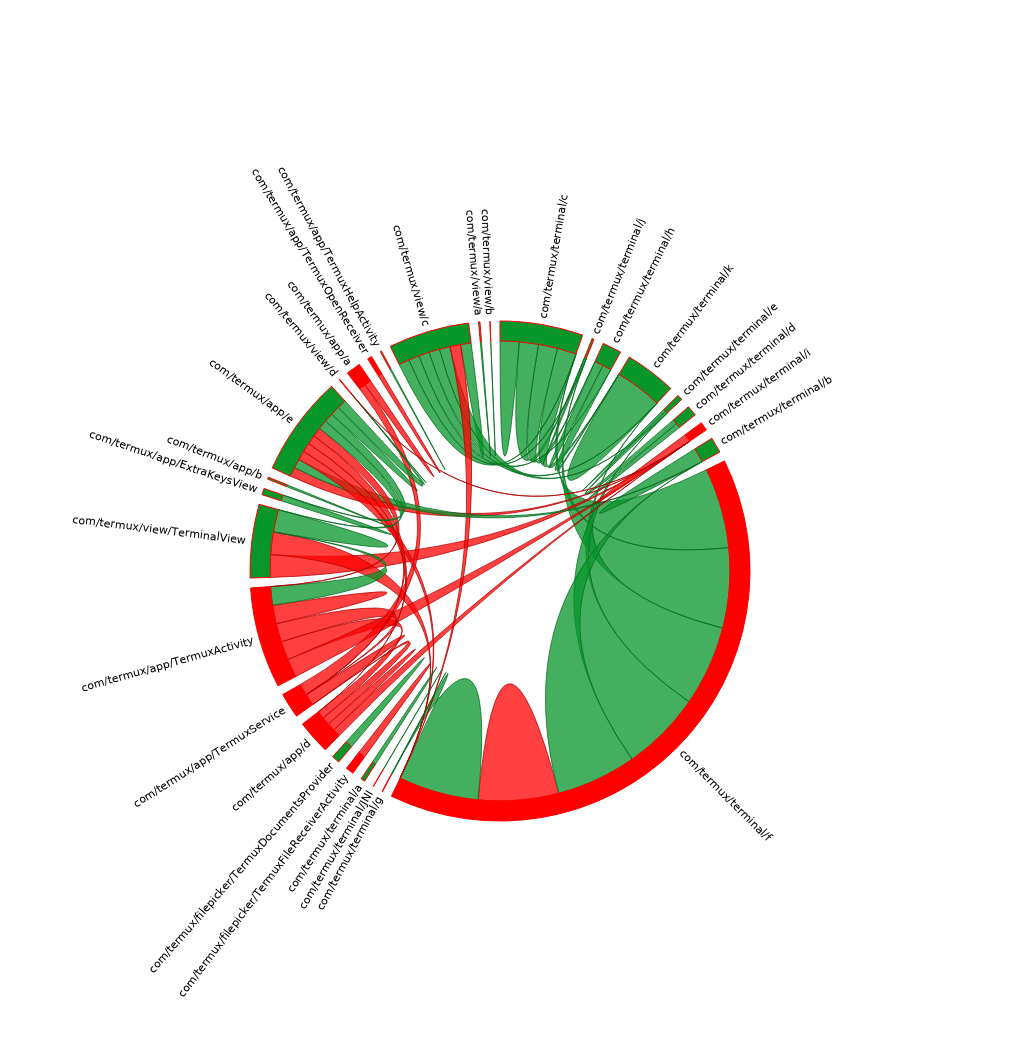
\includegraphics[scale=0.4]{/home/miki/Documents/GITHUB/AndroidPermissions/apks/playstore_apps/com_termux/report/chord_diagram.png}\end{figure}\begin{figure}[H]
\centering
	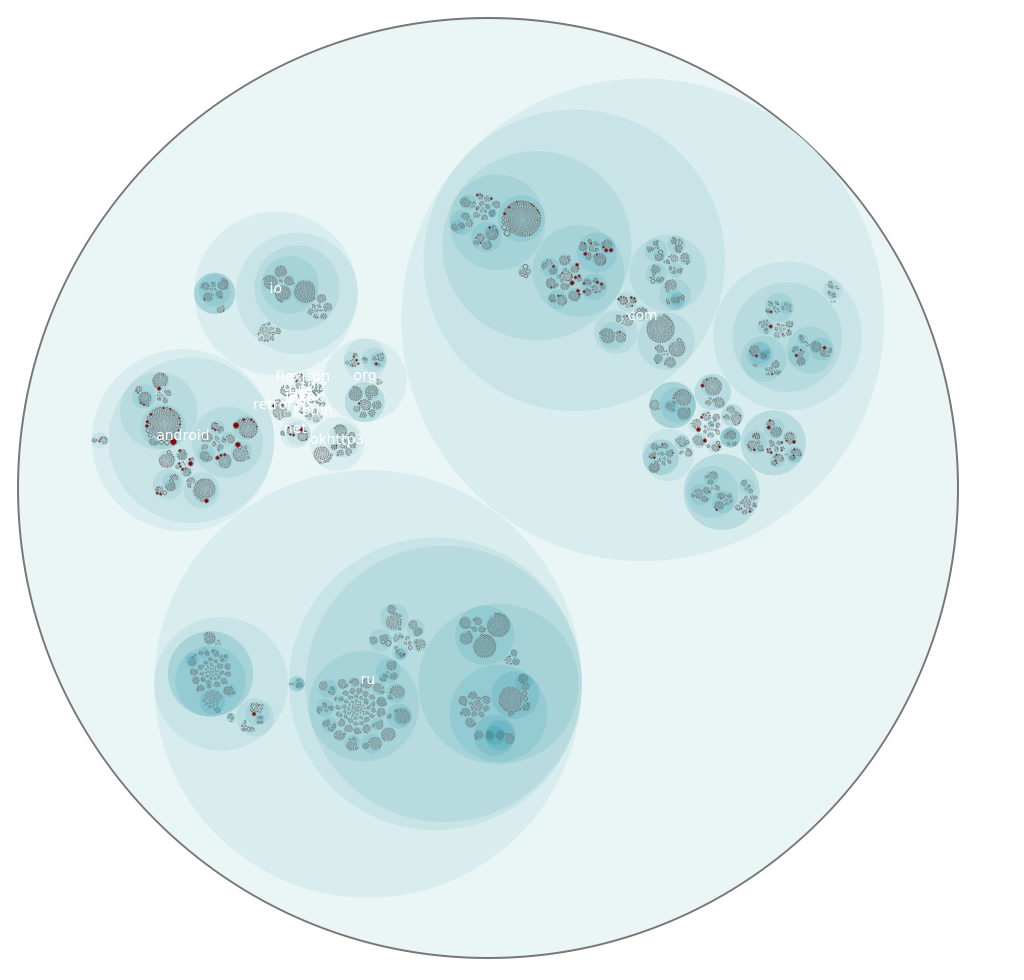
\includegraphics[scale=0.5]{/home/miki/Documents/GITHUB/AndroidPermissions/apks/playstore_apps/com_termux/report/hotspot.png}\end{figure}\begin{longtable}{p{0.5cm} p{10cm}}
\rowcolor{red} Index & Class \\
1 & \path{/home/miki/Documents/GITHUB/AndroidPermissions/apks/playstore_apps/com_termux/app/smali/com/termux/app/TermuxActivity$1.smali} \\
2 & \path{/home/miki/Documents/GITHUB/AndroidPermissions/apks/playstore_apps/com_termux/app/smali/com/termux/app/TermuxActivity$1.smali} \\
3 & \path{/home/miki/Documents/GITHUB/AndroidPermissions/apks/playstore_apps/com_termux/app/smali/com/termux/app/TermuxActivity$1.smali} \\
4 & \path{/home/miki/Documents/GITHUB/AndroidPermissions/apks/playstore_apps/com_termux/app/smali/com/termux/app/TermuxActivity$1.smali} \\
5 & \path{/home/miki/Documents/GITHUB/AndroidPermissions/apks/playstore_apps/com_termux/app/smali/com/termux/app/TermuxActivity$1.smali} \\
6 & \path{/home/miki/Documents/GITHUB/AndroidPermissions/apks/playstore_apps/com_termux/app/smali/com/termux/app/TermuxActivity$1.smali} \\
7 & \path{/home/miki/Documents/GITHUB/AndroidPermissions/apks/playstore_apps/com_termux/app/smali/com/termux/app/TermuxActivity$1.smali} \\
	\end{longtable}
\end{document}
